\section{Materiales y métodos}

Partimos nuestra investigación buscando el interactoma funcional SARS-humano. Aunque el SARS-CoV-2 es un virus reciente, encontramos en la literatura científica numerosos papers que investigan este tema ((\cite{Hoffmann2020}, \cite{Yan2020a}, \cite{Shulla2011}, \cite{Chan2020}, \cite{Gysi2020})). Como podemos ver en \cite{Gysi2020}), el genoma viral del SARS-CoV-2 es capaz de crear 29 proteínas diferentes. En el trabajo \cite{Shulla2011}, Gordon et aI. consiguieron aislar 27 de estas proteínas para estudiar aquellas proteínas humanas que interaccionan con las del SARS-CoV-2. Esta investigación encontró interacciones de proteínas humanas con 26 de las proteínas del SARS-CoV-2. 

Las proteínas humanas que pertenecen al interactoma funcional SARS-humano pueden ser la clave para frenar al virus, impidiendo que éste infecte a las células, se replique y se expanda. Sin embargo, diseñar fármacos específicos para el SARS-CoV-2 puede llevar mucho tiempo, por lo que vamos a estudiar qué fármacos existen actualmente cuya diana sean estas proteínas humanas. 

\subsection{STRING, base de datos de interacción de proteínas}

Como se habla en \cite{Chan2020}, cuando usamos fármacos con dianas específicas, podemos encontrar efectos en proteínas relacionadas. Esta idea se enmarca dentro de la corriente holística, donde debemos estudiar el sistema como un conjunto, en vez de centrarnos en las partes. 

Siguiendo esta reflexión, buscar proteínas que se relacionen directamente con nuestras proteínas diana, que llamaremos proteínas secundarias, y hallar fármacos que actúen sobre estas proteínas secundarias, puede llevarnos a tener tratamientos que indirectamente combatan la acción del virus. 

Para encontrar estas proteínas secundarias, vamos a hacer uso de STRING. STRING es una base de datos de interacciones de proteínas. Introducimos en STRING las proteínas humanas del interactoma SARS-humano que conocemos (un total de 332 proteínas) y hacemos un filtrado de la búsqueda. 

Primero, seleccionamos que la puntuación de la interacción (interaction score) sea de al menos 0.700, lo que nos asegura interacciones de alta confianza. A continuación, pedimos que se nos muestren hasta 100 proteínas que interaccionan con cada una de las introducidas. De esta forma, encontramos las proteínas secundarias para nuestro estudio. 

    \subsubsection{Mapeo de códigos}
    Tras hacer nuestra búsqueda en STRING, tenemos un listado de genes que codifican proteínas del interactoma SARS-Humano (332 genes) y otro listado que corresponde a los genes que codifica a las proteínas secundarias (115 genes).
    
    A continuación, debemos preparar estos datos para nuestro flujo, que requiere que los nombres de los genes se mapeen con el ID de CHEMBL. Este proceso lo hemos hecho usando la herramienta de mapeo Retrieve/ID que proporciona Uniprot. Sin embargo, durante el mapeo, el número de genes disminuye mucho, teniendo finalmente 88 proteínas del interactoma y 30 proteínas secundarias.

\subsection{Código desarrollado}

Para poder obtener los datos de CHEMBL hemos encontrado una serie de paquetes tanto en R como en Python que contienen las funciones deseadas.

\subsubsection{Trabajo en Python}
El principal paquete que existe y tiene acceso a CHEMBL es un cliente web que trabaja a través del lenguaje Python. Su nombre es \textbf{\textit{chembl\_webresource\_client}}, y CHEMBL tiene una sección web dedicada a explicar su funcionamiento. %PONER REFERENCIA

Al usar este paquete se nos presentan dos problemas. El primero es que los datos que obtenemos desde este servicio web no están conectados entre sí de la misma manera en que lo están los datos dentro de CHEMBL. Por tanto, acceder a un medicamento a partir de los targets (proteínas) disponibles no es algo fácil de hacer. El segundo problema se presenta una vez averiguamos cómo hacer esto, y es que los datos descargados no son siempre correctos, y en algunos casos una misma petición devuelve respuestas diferentes en cada ejecución. Esto nos hizo llegar a la conclusión de que no podíamos hacer un programa fiable con este paquete, y por tanto pasamos a otras opciones.

\subsubsection{Trabajo en R}
El paquete que tenemos disponible en R es muy básico, se llama \textbf{\textit{chemblr}} y fue modificado por última vez hace siete años, por lo que no está demasiado actualizado. %PONER REFERENCIA

En vez de basarnos en este paquete, vamos a obtener nuestra información a partir de peticiones GET a la web de CHEMBL. Usaremos de nuevo la página en la que se explica el funcionamiento del servicio web de python, solo que aplicaremos sus ejemplos sobre R. Para hacer esto, nos hemos ayudado de una página de la web de EMBL.  %REFERENCIAS

El paquete \textbf{\textit{chemblr}} lo usaremos simplemente para obtener los json en un formato cómodo. Todos los paquetes requeridos se instalarán en la carpeta \textit{software/deps} dentro de \textit{code}.

\subsubsection{setup.sh}
Para la carga de los distintos paquetes que vamos a usar durante el desarrollo de la actividad, utilizaremos la ventana de comandos. 

Hemos diseñado un script de bash llamado \textbf{\textit{setup.sh}}. En este script, creamos en primer lugar un repositorio local \textbf{deps} que deberá crearse dentro de la carpeta \textbf{software}. 

Antes de proceder a la carga de todas las librerías dentro de este repositorio, concedemos permisos de administrador a la misma. 

Hemos definido dos listas de paquetes, una para aquellos que se obtienen desde CRAN (jsonlite, httr, devtools, sjmisc, tidyverse, networkD3, magrittry) y  otra para aquellos que se obtienen a través del paquete previamente instalado devtools, que en nuestro caso es solo una (chemblr). 

Para cada una de estas listas, ejecutamos un bucle for dentro del cual se instalarán las librerías una por una. 

\subsubsection{launch.sh}
Para ejecutar todo el flujo de trabajo que hemos generado, utilizamos el archivo \textbf{\textit{setup.sh}}. A este archivo le pasamos como argumento un número, que puede ser \textbf{1}, \textbf{2}, \textbf{3} o \textbf{4}. Si le pasamos \textbf{1}, trabajaremos con fármacos en fase 3 y proteínas de primer grado de interacción; en el caso de pasar un \textbf{2}, utilizaremos fármacos en fase 3 y proteínas secundarias; de la misma manera ocurre con el \textbf{3} y el \textbf{4}, a diferencia de que en este caso los fármacos serán de fase 4. 

Este archivo primero cargará todas las librerías que hemos descargado previamente con \textbf{setup.sh} y estarán en la carpeta \textbf{deps} dentro de \textbf{software}. 

Posteriormente, se establecen las variables locales que vamos a usar durante el estudio. Seguidamente se cargan las funciones realizadas y se pasa a la ejecución, donde se utilizan esas funciones. 

Finalmente, se procede a guardar los archivos \textbf{CSV} y las gráficas que hayamos generado durante la actividad en la carpeta \textbf{results}. 


Aquí podemos ver cómo quedaría el flujo: 

\begin{figure}[h!]
			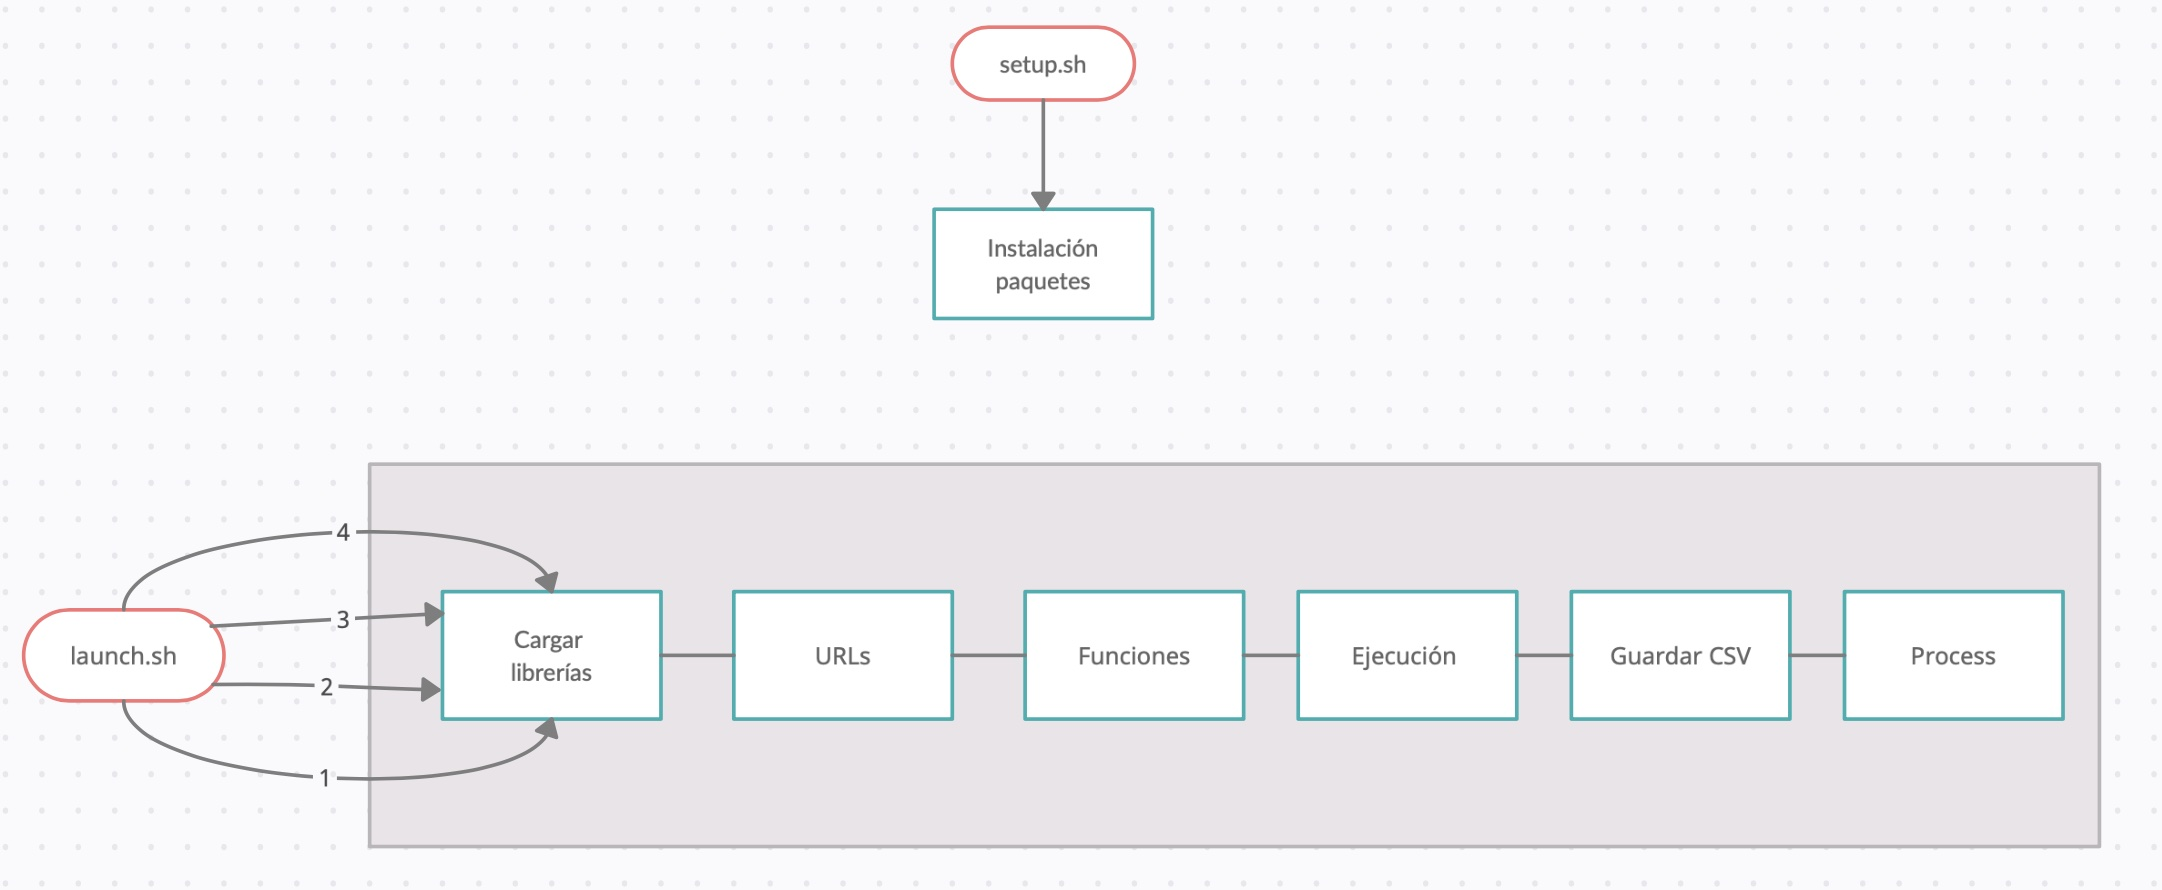
\includegraphics[width=0.9\textwidth]{figures/flujo.jpg}
			\caption{Flujo de trabajo}
		\end{figure}

\newpage